Obvious is a set of interfaces and extension classes for wrapping
around existing information visualization toolkits.  It generalizes
and extend the standard architecture as defined in the Information
Visualization reference model to try to abstract all the existing
implementations.  In this section, we list all of the existing
toolkits and explain what is common and how they differ.  In the
second section, we describe the most common standardization processes
for software systems.

\subsection{Existing toolkits}

Mostly all the existing information visualization toolkits follow the
InfoVis reference model initially specified by Ed Chi and refined by
Card, Mackinlay and Shneiderman~\cite{ChiRefModel,ReadingsIV}.  The
model defines three stages: Data Table, Visual Structure and View
(Figure~\ref{fig:refmodel}).  One of its main value is that is
explicitly represents the interaction, in contrast with older
visualization models.

Several articles have described the concrete design of an information
visualization toolkit.  The InfoVis Toolkit~\cite{InfoVis} is based on
an in-memory database manager where data is organized in columns,
contrary to most relational databases.  The main challenge being the
support of interactive performance for rendering and dynamic queries
with a small memory footprint.  Prefuse~\cite{Prefuse} also relies on
an in-memory database but implements the visual structure as an
extension of the data model (a visual table derives from a data
table).  It then transforms the data into a \emph{polylithic} graphic
structures~\cite{Polylithic} whereas all the other toolkits use a
\emph{monolithic} architecture.


Building upon their experience in the
Prefuse toolkit~\cite{Prefuse}, Heer et Agrawala~\cite{DesignPatternsIV}
presents several software design patterns that are common to
information visualization applications and toolkits.

\begin{figure}
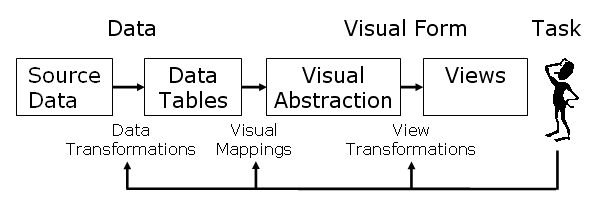
\includegraphics[width=\columnwidth]{figures/reference_model}
\caption{The Information Visualization Reference Model (drawing by
  J. Heer)}
\label{fig:refmodel}
\end{figure}

\cite{DesignPatternsIV}

\subsection{Standardization processes}
ISO, Internet, SQL





